\documentclass[a4paper]{article}

\usepackage{graphicx}
\usepackage{amsmath,amssymb}
\usepackage{minted}
\usepackage{multirow}
\usepackage{float}
\usepackage{algorithm}
\usepackage{algpseudocode}
\usepackage{todonotes}
\usepackage{forest}
\usepackage{xstring}
\usepackage{xcolor}
\usepackage[most]{tcolorbox}
\usepackage{xparse}
\usepackage{natbib}

\usetikzlibrary{graphs,graphdrawing}
\usegdlibrary{layered}

% for external graphviz
\input{/home/donkarlo/Dropbox/repo/nd_language_ai_project/src/nd_language_ai/formal/computer/programming/tex/latex/code_clips/external_graphviz.tex}

% for tags
\input{/home/donkarlo/Dropbox/repo/nd_language_ai_project/src/nd_language_ai/formal/computer/programming/tex/latex/parts/control_sequence/kind/semtag/semtag.tex}

% for links
\input{/home/donkarlo/Dropbox/repo/nd_language_ai_project/src/nd_language_ai/formal/computer/programming/tex/latex/code_clips/seehere.tex}

\title{Preprocessing}
\date{}
\author{Mohammad Rahmani}

\begin{document}
   \maketitle
   Preprocessing is both shared between the training and anomaly detection phase.
   
   \begin{figure}[H]
      \centering
      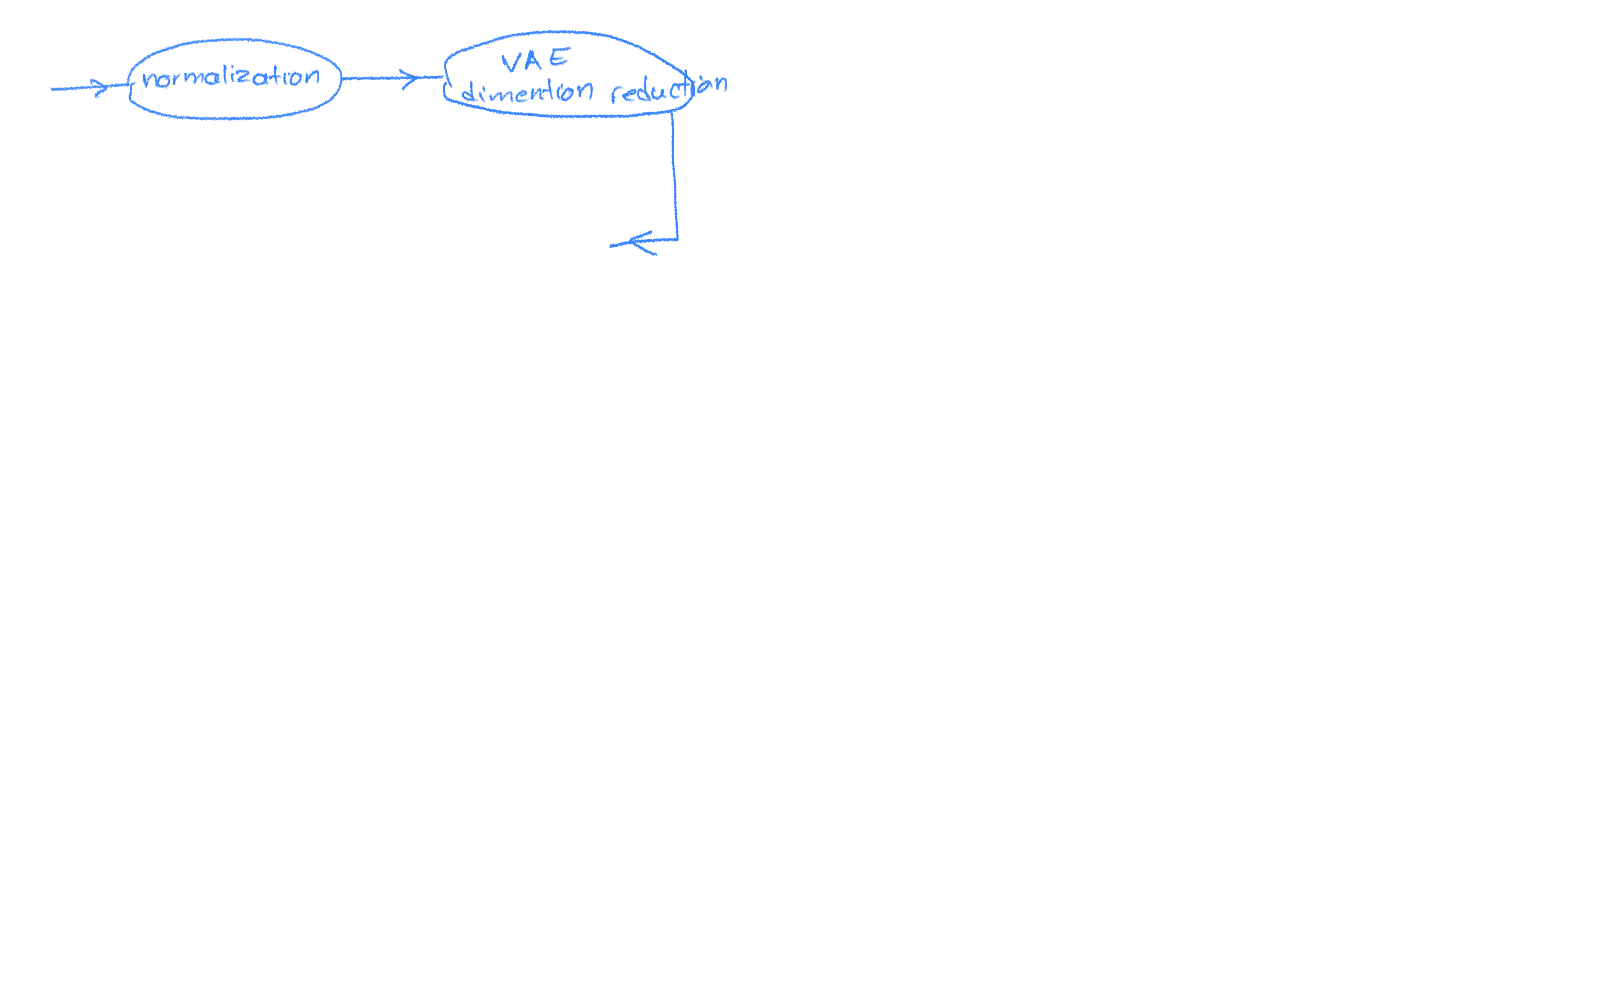
\includegraphics[width=0.9\textwidth]{preprocessing.png}
   \end{figure}
   \section{Nomalisation}
   \section{Dimension reduction VAEs}

      \bibliographystyle{plainnat}
      \bibliography{nd_shared_research/bibliography/bibliography.bib}
\end{document}
